\subsection{Descripción del problema.}

\vspace*{0.3cm}

Tenemos la intención de competir en una versión particular del Rally Dakkar, y para esto decidimos usar nuestros conocimientos en computación a nuestro a favor. Sabemos que en esta competencia podremos usar una BMX, una motocross y un buggy arenero. Nuestro objetivo es finalizar la competencia en el menor tiempo posible, y contamos con los siguientes datos:

\begin{itemize}
	\item El circuito se divide en $n$ etapas (numeradas del 1 al n) y en cada etapa sólo se puede usar un vehículo.
	\item Para cada etapa, se sabe cuánto se tardaría en recorrerla con cada vehículo.
	\item Tanto la motocross como el buggy arenero tienen un número limitado de veces que se pueden usar, a diferencia de la BMX, y estos números son conocidos.
	\item La complejidad del algoritmo pedido es de $\mathcal{O}(n \cdot k_{m} \cdot k_{n})$ donde $n$ es la cantidad de etapas, $k_{m}$ es la cantidad máxima de veces que puedo usar la moto, y $k_{b}$ la cantidad máxima de veces que puedo usar el buggy.
	\item La salida de este algoritmo deberá mostrar el tiempo total de finalización de la carrera y una sucesión de $n$ enteros representando el vehículo utilizado en cada etapa (1 para bici, 2 para moto y 3 para buggy).
\end{itemize}

Ejemplo:

Supongamos un Rally de 3 etapas, en donde puedo usar una vez la moto y una vez el buggy, con los siguientes datos:

\begin{table}[!ht]
\begin{center}
\begin{tabular}{| c | c | c | c |}
\hline
Etapa & BMX & Moto & Buggy\\
\hline
1 & 10 & 8 & 7\\
\hline
2 & 8 & 3 & 7\\
\hline
3 & 15 & 6 & 2\\
\hline
\end{tabular}
\end{center}
\end{table}

Con estos datos, la manera óptima de llevar a cabo la carrera sería la siguiente:

\begin{table}[!ht]
\begin{center}
\begin{tabular}{| c | c | c | c |}
\hline
Etapa 1 & Etapa 2 & Etapa 3 & Tiempo total\\
BMX: 10 & Moto: 3 & Buggy: 2 & 15\\
\hline
\end{tabular}
\end{center}
\end{table}

\vspace*{0.6cm}
%\newpage
\subsection{Desarrollo de la idea y correctitud.}

\vspace*{0.3cm}

LLamemos $n$ a la cantidad de etapas del Rally, $k_{m}$ y $k_{b}$ a la cantidad máxima de motos y buggys respectivamente que es posible utilizar en el Rally. La idea es no tratar de resolver todas las etapas de un tirón, sino tratar primero de resolver considerando sólo la primer etapa, luego considerando las dos primeras etapas ayudándonos con la resolución de la primera etapa sola, luego considerando las primeras tres etapas ayudándonos con la resolución de las primeras dos etapas, y así hasta llegar a considerar $n$ etapas. Para esto, la resolución que considera las primeras $h$ etapas tendrá una tabla construida a partir de la información de la tabla correspondiente a la resolución de las primeras $h-1$ etapas. Cada una de estas tablas tiene $k_{m}+1$ columnas (numeradas del $0$ al $k_{m}$) y $k_{b}+1$ filas (numeradas del $0$ al $k_{b}$). Para hacer referencia a la tabla que representa a las primeras $t$ etapas (con $t$ algún número natural distinto de 0), la llamaremos la tabla $t$.  Entonces si tomamos $i,j,h \in \mathbb{N}$ tal que $0 \leq i \leq k_{b}$, $0 \leq j \leq k_{m}$ y $1 \leq h \leq n$ la idea sería que la posición $i,j$ de la tabla $h$ tenga dos datos: el tiempo óptimo de las primeras $h$ etapas usando a lo sumo $i$ buggies y $j$ motos, y el vehículo que se usaría en la etapa $h$ bajo esas circunstancias. 

Determinemos ahora cómo se completarían las tablas (para hacer referencia a una posición de una tabla $h$, diremos la posición $h_{f,c}$ donde $f$ es el número de fila, y $c$ el número de columna):

\begin{itemize}
	\item Si $h = 1$
	\begin{itemize}
		\item En la posición $h_{0,0}$ colocaremos el tiempo de la bicicleta en la etapa $h$, puesto que sólo puede usarse ese vehículo, e indicaremos que se usó la bici.
		\item En la posición $h_{0,1}$ colocaremos el tiempo de la bicicleta o la moto (ambos en la etapa $h$), el que sea menor, e indicaremos cuál de ellos se utilizó.
		\item De la posición $h_{0,2}$ hasta $h_{0,k_{m}}$ colocaremos exactamente lo que hay en $h_{0,1}$ dado que si consideramos una sola etapa, poder usar una moto o más de una, no es diferencia.
		\item En la posición $h_{1,0}$ colocaremos el tiempo de la bicicleta o el buggy (ambos de la etapa $h$), el que sea menor, e indicaremos cuál de ellos se utilizó.
		\item De la posición $h_{2,0}$ hasta $h_{k_{b},0}$ colocaremos exactamente lo que hay en $h_{1,0}$ dado que si consideramos una sola etapa, poder usar un buggy o más de uno, no es diferencia.
		\item En la posición $h_{1,1}$ colocaremos el tiempo de la bicicleta, el buggy o la moto (de la etapa $h$), el que sea menor, e indicaremos cuál de ellos se utilizó.
		\item El resto de las posiciones de esa tabla, deben tener lo que hay en $h_{1,1}$ dado que si tengo una sola etapa, poder usar una moto y un buggy, o más de alguno de ellos o de ambos, no es diferencia.
	\end{itemize}

	\item Para todo $h$ tal que $1 < h \leq n$
	\begin{itemize}
		\item En la posición $h_{0,0}$ colocaremos el tiempo que de la posición $(h-1)_{0,0}$ sumada al de la bici de la etapa $h$, e indicaremos que se usó la bici. El tiempo óptimo de este caso es correcto, puesto que al no poder usar otros vehículos, el tiempo óptimo de haber recorrido $h$ etapas usando solo la bicicleta, es el tiempo óptimo de haber recorrido $h-1$ etapas sin usar buggys ni motos, sumado a usar una bicicleta en la etapa $h$. El vehículo elegido es trivialmente correcto, puesto que no hay otra elección posible. 
		\item Tomando $1 \leq j \leq k_{m}$, la posición $h_{0,j}$ debe contener el tiempo mínimo entre:
		\begin{enumerate}
			\item El tiempo de $(h-1)_{0,j}$ sumado al tiempo de la bici en la etapa $h$.
			\item El tiempo de $(h-1)_{0,(j-1)}$ sumado al tiempo de la moto en la etapa $h$.
		\end{enumerate} 
		Para el primer caso indicaremos que se eligió la bici, y para el segundo caso indicaremos que se eligió la moto. Veamos que el tiempo escogido es óptimo:
		\begin{enumerate}
			\item Si el vehículo que deberíamos tomar en la etapa $h$ fuera la bicicleta, entonces en las primeras $h-1$ etapas pudimos haber usado hasta $j$ motos (dado que no vamos a usar ninguna moto en esta etapa).  Como $(h-1)_{0,j}$ indica el tiempo óptimo de usar hasta $j$ motos en las primeras $h-1$ etapas, al sumarle el tiempo de utilizar la bicicleta en la etapa $h$ obtenemos el tiempo óptimo para esta etapa.
			\item Si el vehículo que deberíamos tomar en la etapa $h$ fuera la moto, entonces en las primeras $h-1$ etapas pudimos haber usado hasta $j-1$ motos (dado que vamos a usar una moto en esta etapa).  Como $(h-1)_{0,(j-1)}$ indica el tiempo óptimo de usar hasta $j-1$ motos en las primeras $h-1$ etapas, al sumarle el tiempo de utilizar la moto en la etapa $h$ obtenemos el tiempo óptimo para esta etapa.
		\end{enumerate}
		Como tomamos el mínimo entre 1) y 2) entonces, y ambos, de ser la respuesta correcta, serían óptimos, entonces la elección resulta óptima en tiempo. Por esto mismo, el vehículo elegido es el correcto. Ver que no se crean conflictos con el buggy, ni tenemos que considerar elegirlo o no, puesto que no podemos usar buggies en estos casos.
		\item Tomando $1\leq i \leq k_{b}$ la posición $h_{i,0}$ debe contener el tiempo mínimo entre:
		\begin{enumerate}
			\item El tiempo de $(h-1)_{i,0}$ sumado al tiempo de la bici en la etapa $h$.
			\item El tiempo de $(h-1)_{(i-1),0}$ sumado al tiempo del buggy en la etapa $h$.
		\end{enumerate} 
		Para el primer caso indicaremos que se eligió la bici, y para el segundo caso indicaremos que se eligió el buggy. Veamos que el tiempo escogido es óptimo:
		\begin{enumerate}
			\item Si el vehículo que deberíamos tomar en la etapa $h$ fuera la bicicleta, entonces en las primeras $h-1$ etapas pudimos haber usado hasta $i$ buggies (dado que no vamos a usar ningún buggy en esta etapa).  Como $(h-1)_{i,0}$ indica el tiempo óptimo de usar hasta $i$ buggies en las primeras $h-1$ etapas, al sumarle el tiempo de utilizar la bicicleta en la etapa $h$ obtenemos el tiempo óptimo para esta etapa.
			\item Si el vehículo que deberíamos tomar en la etapa $h$ fuera el buggy, entonces en las primeras $h-1$ etapas pudimos haber usado hasta $i-1$ buggies (dado que vamos a usar un buggy en esta etapa).  Como $(h-1)_{(i-1),0}$ indica el tiempo óptimo de usar hasta $i-1$ buggies en las primeras $h-1$ etapas, al sumarle el tiempo de utilizar un buggy en la etapa $h$ obtenemos el tiempo óptimo para esta etapa.
		\end{enumerate}
		Como tomamos el mínimo entre 1) y 2) entonces, y ambos, de ser la respuesta correcta, serían óptimos, entonces la elección resulta óptima en tiempo. Por esto mismo, el vehículo elegido es el correcto. Ver que no se crean conflictos con la moto, ni tenemos que considerar elegirla o no, puesto que no podemos usar motos en estos casos.
		\item Tomando $1 \leq i \leq k_{b}$ y $1 \leq j \leq k_{m}$ la posición $h_{i,j}$ debe contener el tiempo mínimo entre:
		\begin{enumerate}
			\item El tiempo de $(h-1)_{i,j}$ sumado al tiempo de la bici en la etapa $h$.
			\item El tiempo de $(h-1)_{i,(j-1)}$ sumado al tiempo de la moto en la etapa $h$.
			\item El tiempo de $(h-1)_{(i-1),j}$ sumado al tiempo del buggy en la etapa $h$.
		\end{enumerate} 
		Para el primer caso indicaremos que se eligió la bici, para el segundo caso indicaremos que se eligió la moto y para el tercer caso indicaremos que se eligió el buggy. Veamos que el tiempo escogido es óptimo:
		\begin{enumerate}
			\item Si el vehículo que deberíamos tomar en la etapa $h$ fuera la bicicleta, entonces en las primeras $h-1$ etapas pudimos haber usado hasta $i$ buggies y $j$ motos (dado que no vamos a usar ningún buggy ni moto en esta etapa).  Como $(h-1)_{i,j}$ indica el tiempo óptimo de usar hasta $i$ buggies y hasta $j$ motos en las primeras $h-1$ etapas, al sumarle el tiempo de utilizar la bicicleta en la etapa $h$ obtenemos el tiempo óptimo para esta etapa.
			\item Si el vehículo que deberíamos tomar en la etapa $h$ fuera la moto, entonces en las primeras $h-1$ etapas pudimos haber usado hasta $j-1$ motos y hasta $i$ buggies (dado que vamos a usar una moto en esta etapa).  Como $(h-1)_{i,(j-1)}$ indica el tiempo óptimo de usar hasta $i$ buggies y hasta $j-1$ motos en las primeras $h-1$ etapas, al sumarle el tiempo de utilizar la moto en la etapa $h$ obtenemos el tiempo óptimo para esta etapa.
			\item Si el vehículo que deberíamos tomar en la etapa $h$ fuera el buggy, entonces en las primeras $h-1$ etapas pudimos haber usado hasta $i-1$ buggies y hasta $j$ motos (dado que vamos a usar un buggy en esta etapa).  Como $(h-1)_{(i-1),j}$ indica el tiempo óptimo de usar hasta $i-1$ buggies y hasta $j$ motos en las primeras $h-1$ etapas, al sumarle el tiempo de utilizar un buggy en la etapa $h$ obtenemos el tiempo óptimo para esta etapa.
		\end{enumerate}
		Como tomamos el mínimo entre 1), 2) y 3), y todos, de ser la respuesta correcta, serían óptimos, entonces la elección resulta óptima en tiempo. Por esto mismo, el vehículo elegido es el correcto.
	\end{itemize}
\end{itemize}

	Entonces, una vez completas las tablas, si queremos saber cuál es el menor tiempo en el que podemos completar el Rally, tan sólo debemos ver el tiempo de $n_{k_{b},k_{m}}$, y si queremos saber qué vehículos utilizamos en cada etapa, debemos ver qué vehículo se usó en $n_{k_{b},k_{m}}$ y ese vehículo será el que se usó en la etapa $n$. Luego, de manera general, suponiendo $2 \leq h \leq n$, para extraer el vehículo utilizado en la etapa $h-1$, habiendo extraído el vehículo de la etapa $h$ de la posición $h_{i,j}$ con $0\leq i \leq k_{b}$ y $0\leq j \leq k_{m}$, por cómo está hecha la tabla, debemos ir a:
	
\begin{itemize}
	\item la posición $(h-1)_{i,j}$ si en la etapa $h$ elegimos la bici.
	\item la posición $(h-1)_{i,j-1}$ si en la etapa $h$ elegimos la moto.
	\item la posición $(h-1)_{i-1,j}$ si en la etapa $h$ elegimos el buggy.
\end{itemize}			

	 Y en la posición a la que haya ido, extraer el vehículo utilizado, que será el correspondiente a la etapa $h-1$. Haciendo esto en orden, se obtendría qué vehículo fue utilizado en cada etapa. De esta manera, se resolvería el problema de manera correcta.
 
\vspace*{0.6cm}

%\newpage

\subsection{Análisis de complejidad.}

\vspace*{0.3cm}

Para empezar a analizar la complejidad de nuestro algoritmo veamos brevemente cómo funciona la función {\sc Elección}. Ésta, por medio de una serie de simples comparaciones entre los tiempos de la bicicleta, la moto y el buggy en $\mathcal{O}(1)$, devuelve el valor y el vehículo que, para la etapa en cuestión, resultan óptimos.

Partiendo de esta base, observemos que nuestro algoritmo se encarga de rellenar $n$ tablas de tamaño $km*kb$, haciendo uso de {\sc Elección}, cuya complejidad ya dijimos, es $\mathcal{O}(1)$. En consecuencia, este proceso posee una complejidad de $\mathcal{O}(n*km*kb)$.

Hasta aquí hemos cubierto la función {\sc Dakkar} (Figura \ref{code:dakkar}), la cual como veremos en breve, es la que termina asginando la complejidad total del algoritmo planteado. Esto se debe a que, una vez completadas las $n$ tablas, el tiempo total incurrido se obtiene accediendo a la posición $(kb,km)$ de la última tabla generada, y luego se recorre, dependiendo de la elección del vehículo, una casilla determinada de cada tabla ``etapa'', agregando el vehículo utilizado en la lista solución. Como tenemos $n$ tablas y tanto acceder a una posición de una tabla como agregar elementos al principio de una lista es $\mathcal{O}(1)$, este proceso toma $\mathcal{O}(n)$.

A continuación, mostramos el resultado, que consiste en recorrer una lista de $n$ elementos y mostrar cada uno de estos en $\mathcal{O}(1)$ (Figura \ref{code:dakkar.salida}).

Para concluir, sea $T(n)$ la complejidad de nuestro algoritmo, tenemos:

\begin{equation*}
\begin{array}{l}
T(n) = \mathcal{O}(n*km*kb) + 2\mathcal{O}(n)\\
T(n) = \mathcal{O}(n*km*kb)
\end{array}
\end{equation*}

Observemos que, por como se planteó nuestra solución, la complejidad en ``mejor caso'' y en ``peor caso'' de nuestro algoritmo son iguales. Esto sucede ya que en cualquier caso que se plantee, la función {\sc Dakkar}, que por lo dicho anteriormente es la que termina asignando la complejidad de la función, debe rellenar $n$ veces tablas de $km*kb$.

%CHEEEEE, NO HABIA UNA FUNCION ELLECCION EN PSEUDO, O YO FLASHIE XD?? (ALE) 
%Antes de terminar, es necesario aclarar que, por como se planteo nuestra solución, no podríamos un caso que resultara mas ventajoso que otro. Esto sucede ya que en cualquier caso que se plantee los pasos a realizar son los mismos. Por ende la complejidad que estamos planteando aplica para tanto para ``mejor caso'' como para ``peor caso''.\\

\begin{figure}[!ht]
\begin{codebox}
\Procname{$\proc{Dakkar}(n,km,kb,bicis,motos,buggies)$}
\li $etapa_1(0,0) \leftarrow$ [bicis_1,bici]
\li \For $j = 1$ to $km$
\li 		\Do $etapa_1(0,j) \leftarrow$ {\sc Elección}(bicis_1,motos_1)
		\End
\li \For $i = 1$ to $kb$
\li 		\Do $etapa_1(i,0) \leftarrow$ {\sc Elección}(bicis_1,buggies_1)
		\End		
\li \For $i = 1$ to $kb$
\li 		\Do 
		\For $j = 1$ to $km$
\li			\Do $etapa_1(i,j) \leftarrow$ {\sc Elección}(bicis_1,motos_1,buggies_1)
			\End
		\End
\li \For $h = 1$ to $n$
\li 		\Do 
			$etapa_h(0,0) \leftarrow$ [$etapa_{h-1}(0,0)$+bicis_h, bici]
\li 			\For $j = 1$ to $km$
\li 				\Do $etapa_h(0,j) \leftarrow$ {\sc Elección}($etapa_{h-1}(0,j)$ + bicis_h,$etapa_{h-1}(0,j-1)$ + motos_h)
				\End
\li 			\For $i = 1$ to $kb$
\li 				\Do $etapa_h(i,0) \leftarrow$ {\sc Elección}($etapa_{h-1}(i,0)$ + bicis_h,$etapa_{h-1}(i-1,0)$ + buggies_h)
				\End
\li 			\For $i = 1$ to $kb$
\li 				\Do
				\For $j = 1$ to $km$
\li	 				\Do $etapa_h(i,j) \leftarrow$ {\sc Elección}($etapa_{h-1}(i,j)$ + bicis_h,$etapa_{h-1}(i,j-1)$ + motos_h,\\ \hspace*{10cm} $etapa_{h-1}(i-1,j)$ + buggies_h)
					\End
				\End
		\End
\end{codebox} 
\caption{Pseudocódigo del algoritmo para Dakkar}\label{code:dakkar}
\end{figure}
\FloatBarrier

\begin{figure}[!ht]
\begin{codebox}
\Procname{$\proc{Dakkar_salida}(etapas,km,kb)$}
\li i $\leftarrow$ kb
\li j $\leftarrow$ km
\li res $\leftarrow$ lista vacía de vehículos
\li mostrar tiempo_total $\leftarrow etapa_n(i,j).tiempo$
\li \For $h = n$ to 1
\li 		\Do 
			vehículo $\leftarrow etapa_h(i,j).vehiculo$
\li			res $\leftarrow$ agregar vehículo al principio
\li			\If vehículo == moto
\li				\Do decrementar j
\li 			\Else \If vehículo == buggy
\li					\Do decrementar i
					\End
			\End
		\End
\li Recorrer la lista res y mostrar los elementos
\end{codebox} 
\caption{Pseudocódigo del armado de la salida de Dakkar}\label{code:dakkar.salida}
\end{figure}
%\FloatBarrier

\vspace*{0.6cm}
%\newpage
\subsection{Experimentación y gráficos.}

\vspace*{0.3cm}

\subsubsection{Test 1}

\begin{figure}[htb]
	\begin{center}
    		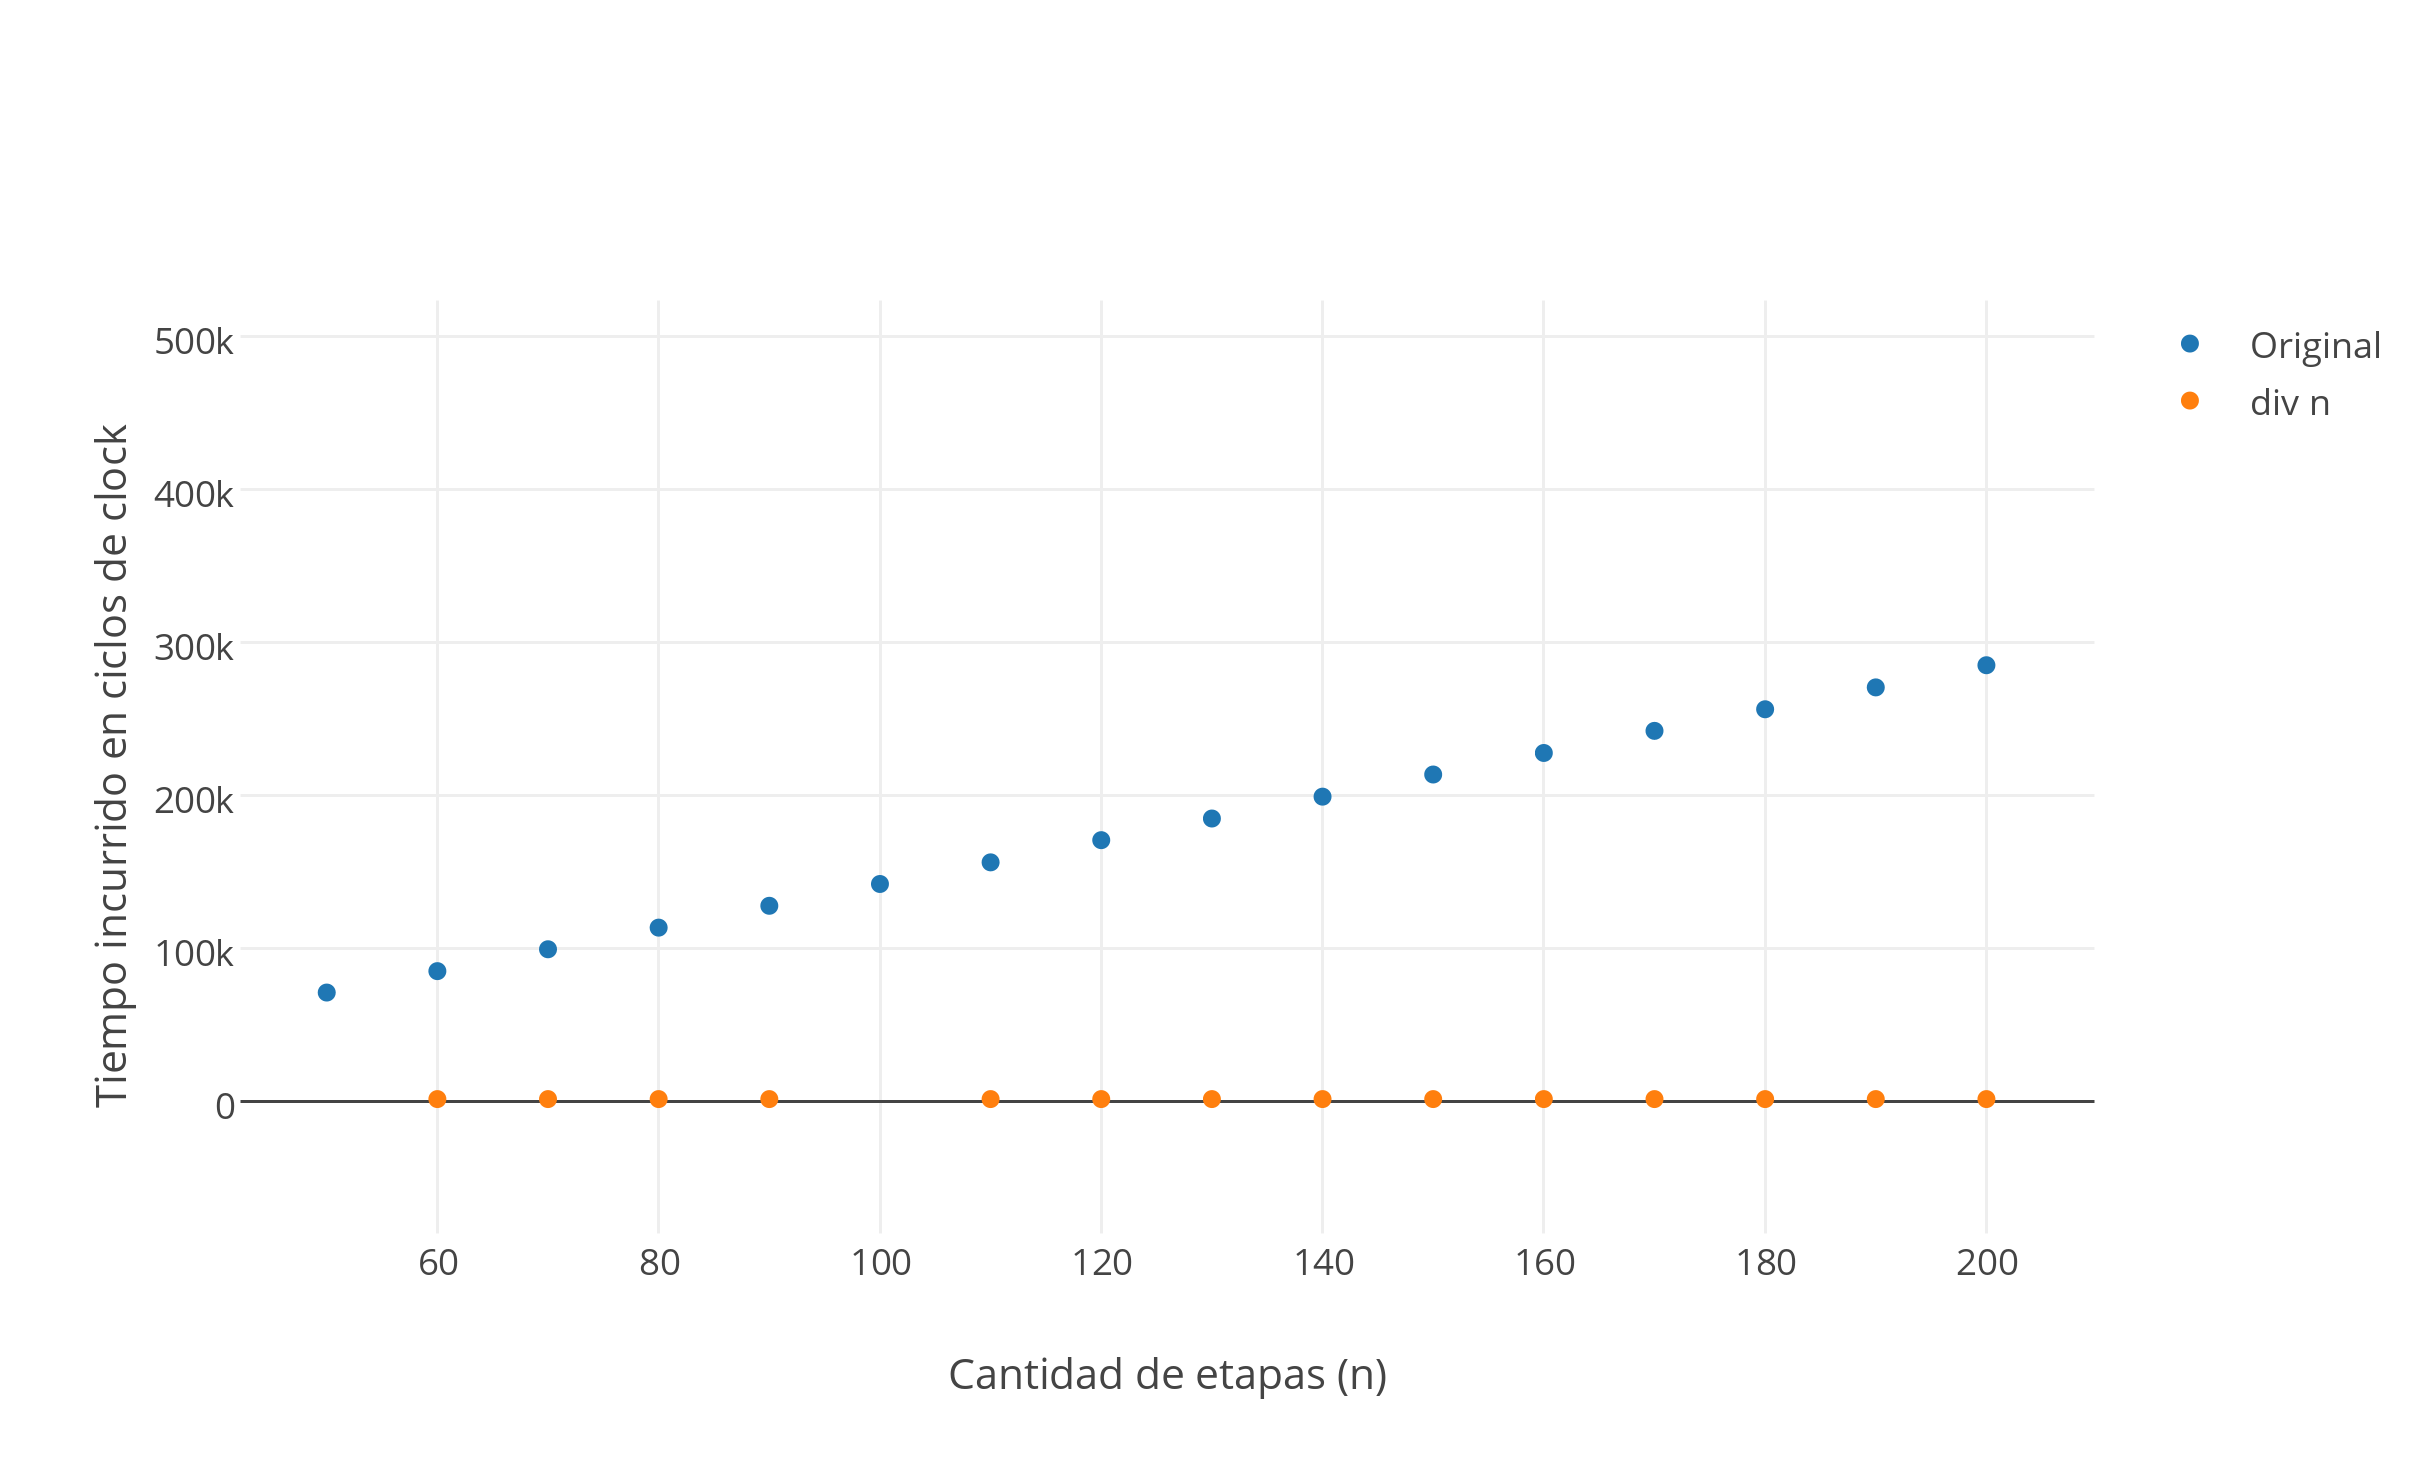
\includegraphics[scale=0.5]{imagenes/1A.png}
	\end{center}
	\caption{Dakkar - Complejidad con etapas variables}\label{fig:1A}
\end{figure}

\begin{figure}[htb]
	\begin{center}
    		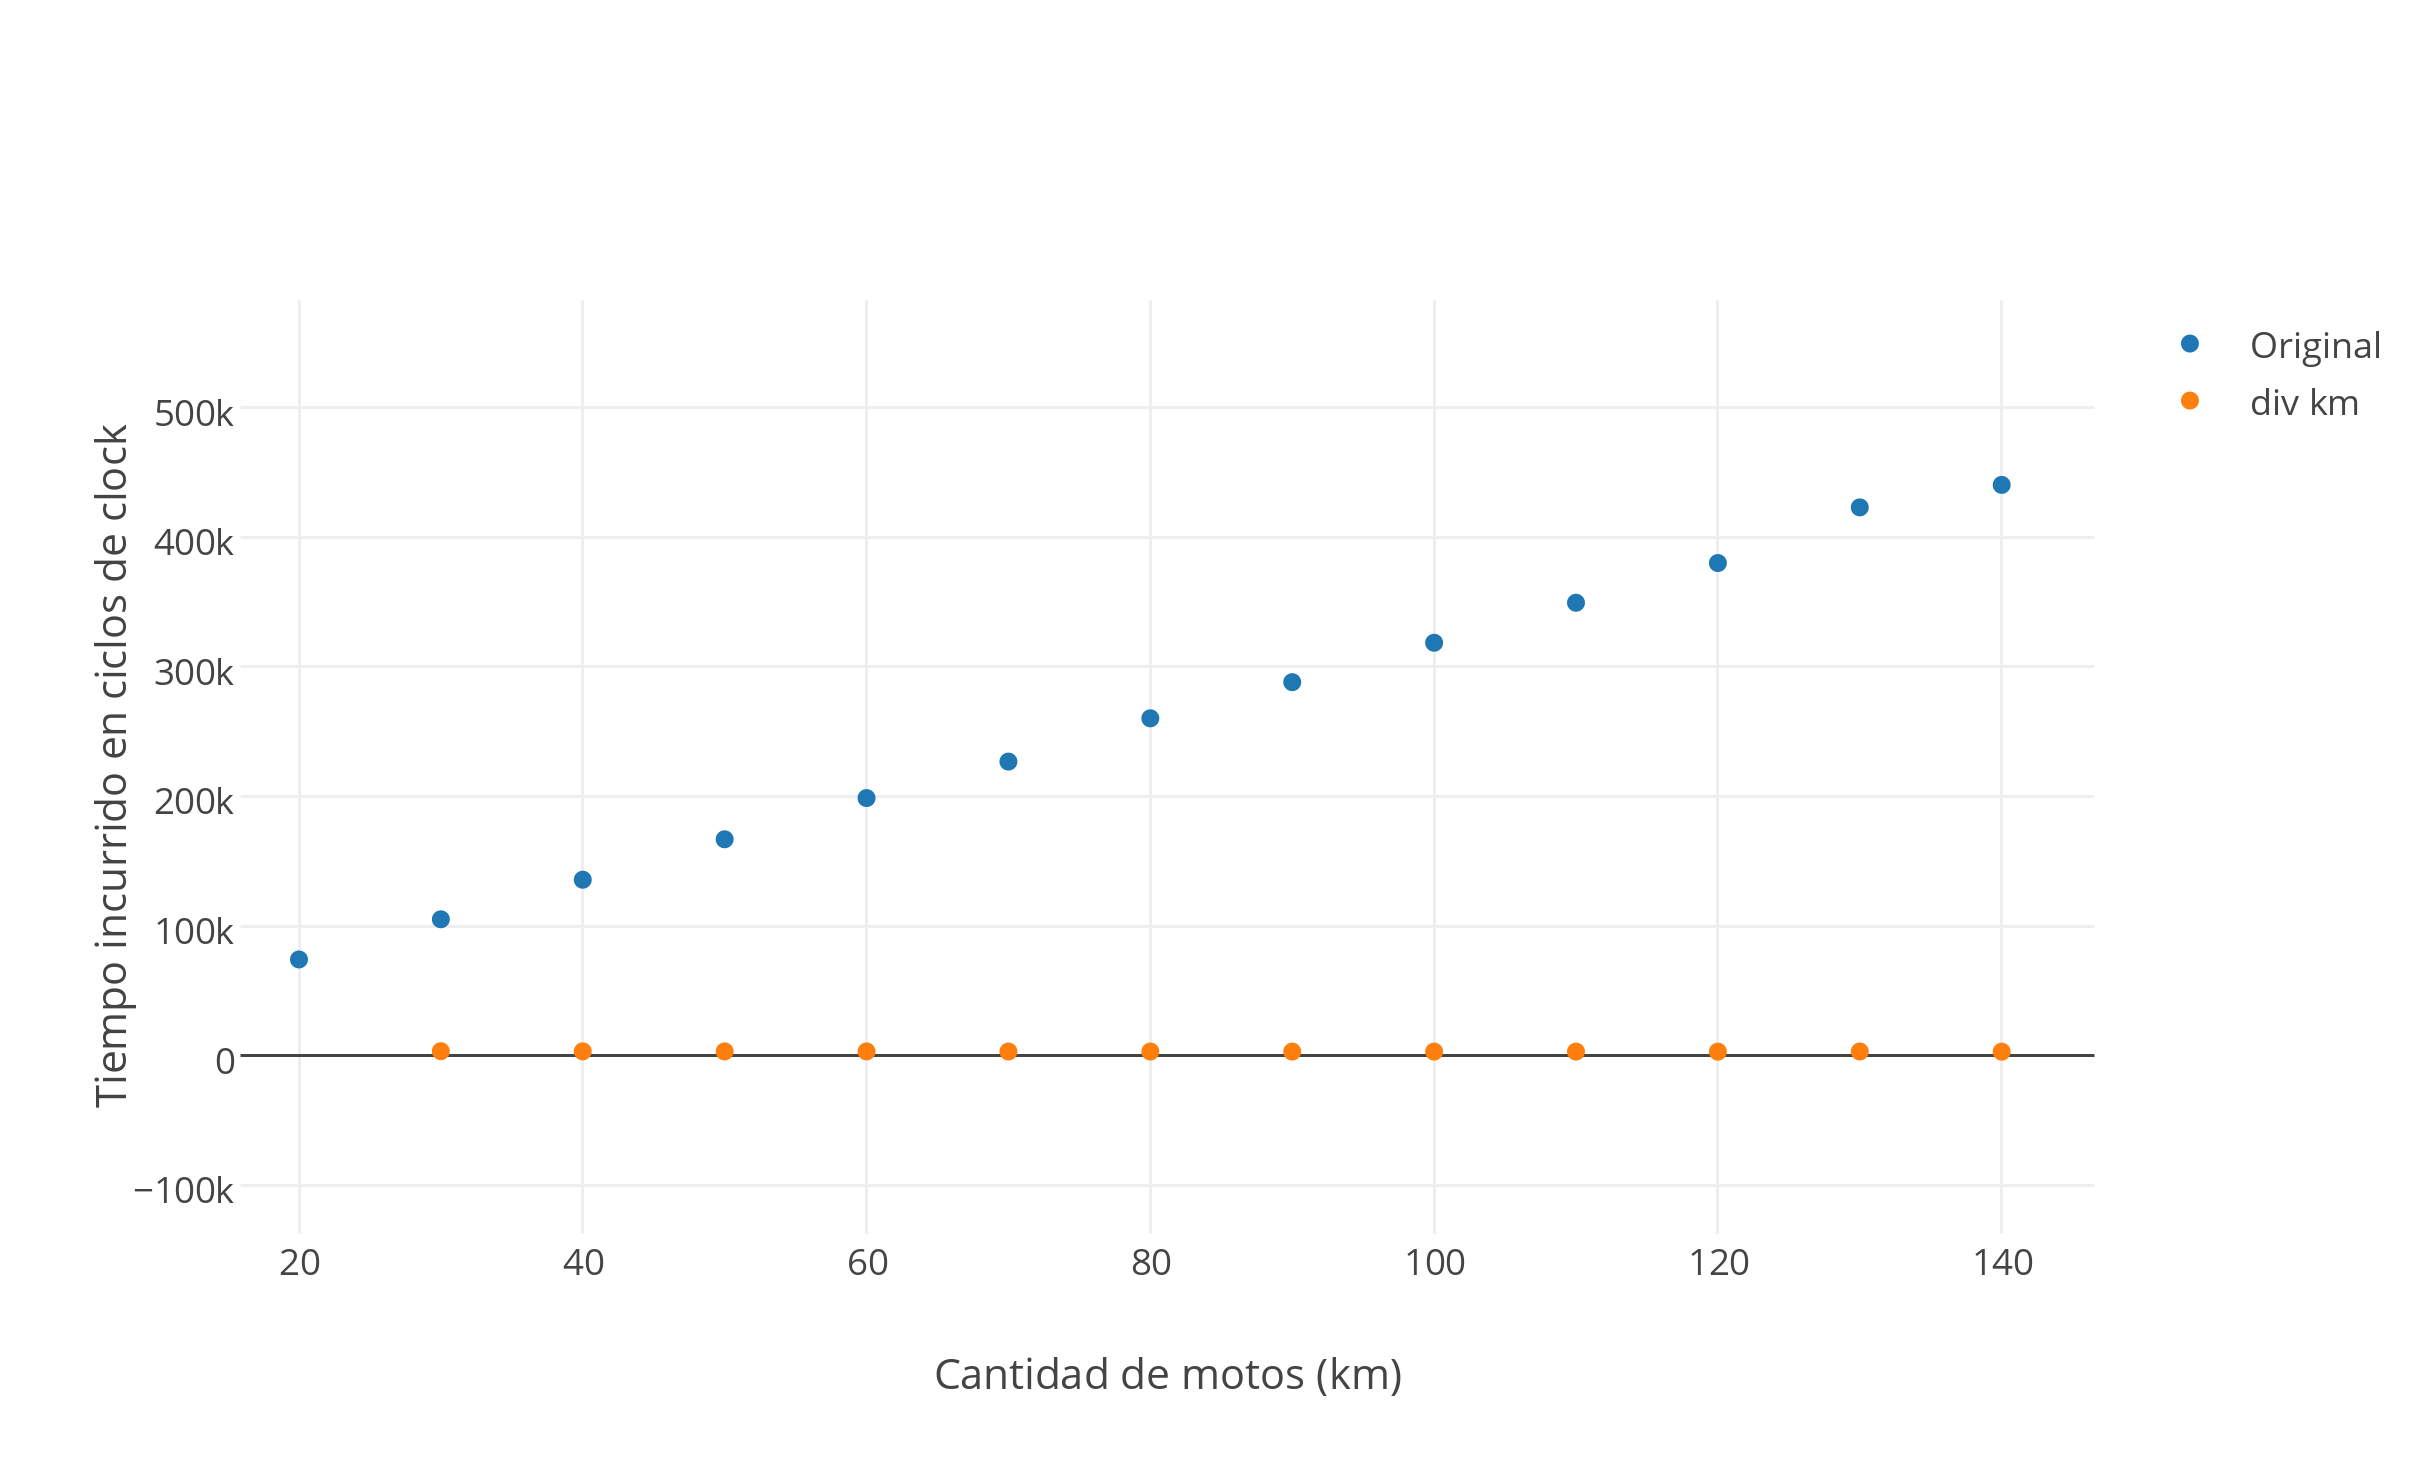
\includegraphics[scale=0.5]{imagenes/1B km.png}
	\end{center}
	\caption{Dakkar - Complejidad con motos variables}\label{fig:1B}
\end{figure}

\begin{figure}[htb]
	\begin{center}
    		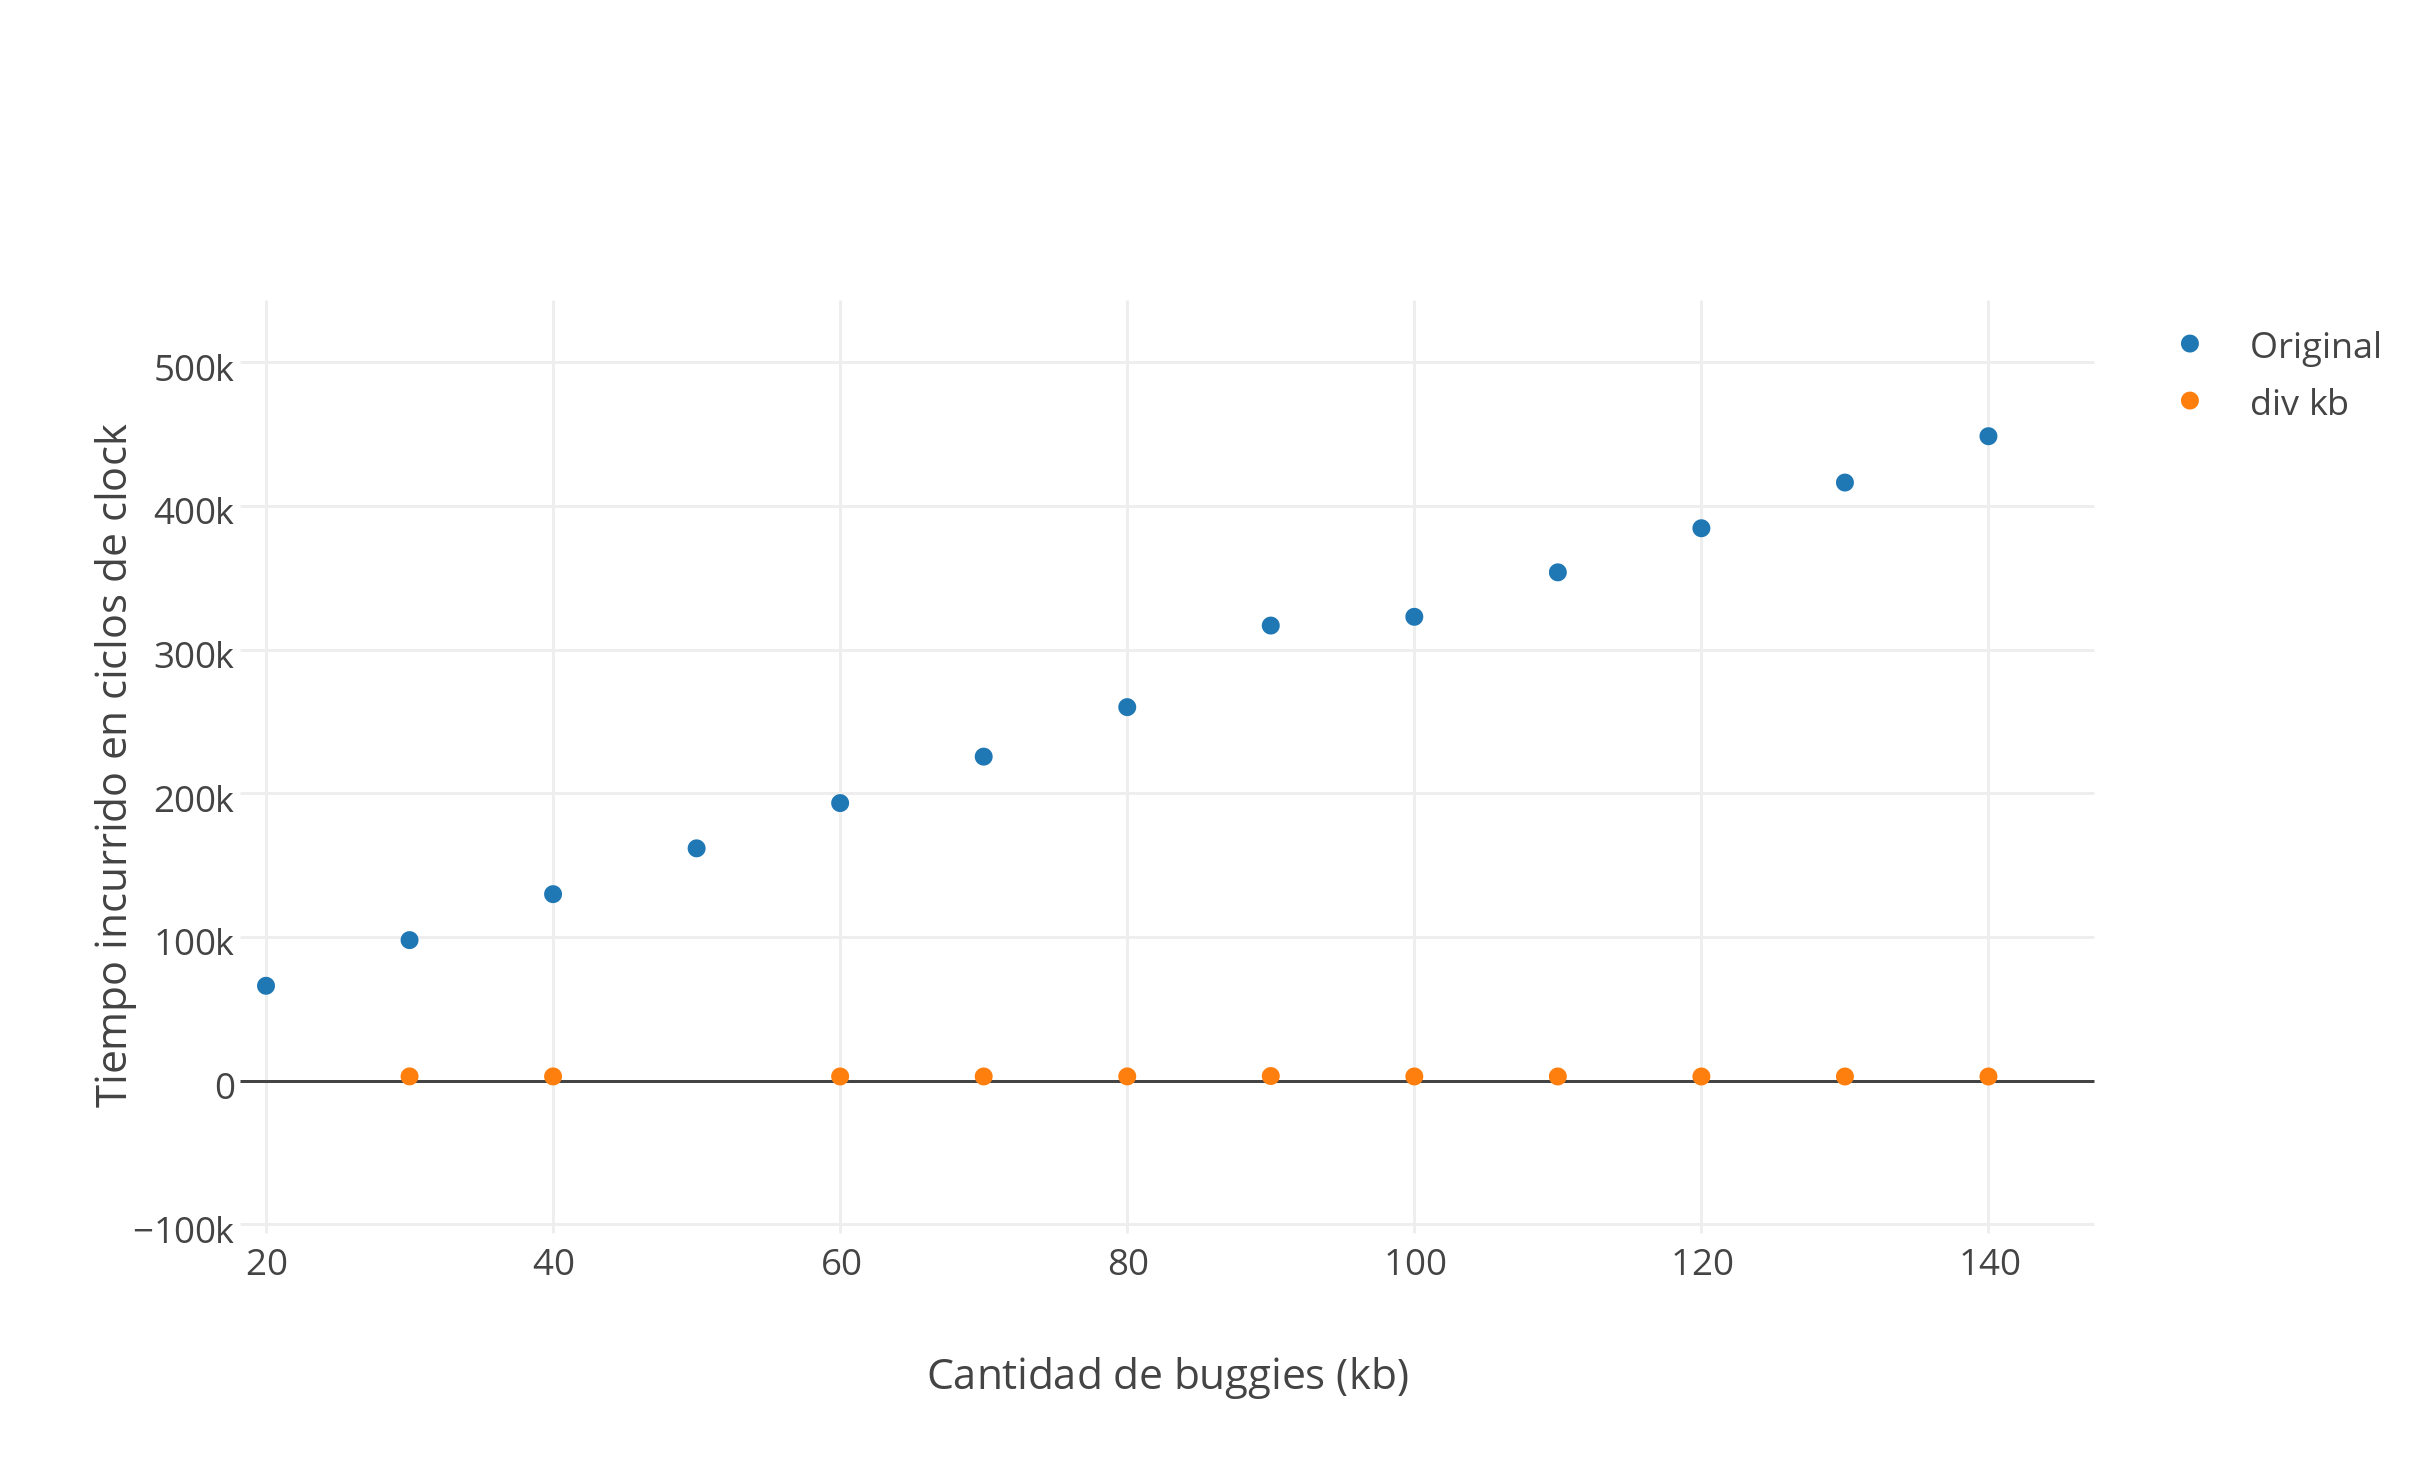
\includegraphics[scale=0.5]{imagenes/1B kb.png}
	\end{center}
	\caption{Dakkar - Complejidad con buggies variables}\label{fig:1C}
\end{figure}

Podemos observar en la figura \ref{fig:1A} ,y en figura (la que muestra como crecen buggys y motos) teniendo en cuenta las tres variables, cantidad de etapas, cantidad de buggies y cantidad de motos, al dejar constante dos de ellas, el tiempo que incurre la tercera parecería ser lineal dado que estaríamos observando una recta. Para poder fundamentar que lo que vemos es en efecto, una recta, los gráficos () toman la variable libre(llamemosla n), y dividen el tiempo incurrido por n. Dado que el resultado en ellos es una constante, podemos afirmar en base a estos, que si dejamos dos variables constantes, la tercera crece de forma lineal. Como consecuencia de esto, se ve reafirmado el analisis teórico, y que nuestro algoritmo tiene complejidad temporal $\mathcal{O}(n*km*kb)$



\vspace*{0.3cm}

\vspace*{0.6cm}
%\newpage

\subsubsection{Test 2}

\begin{figure}[htb]
	\begin{center}
    		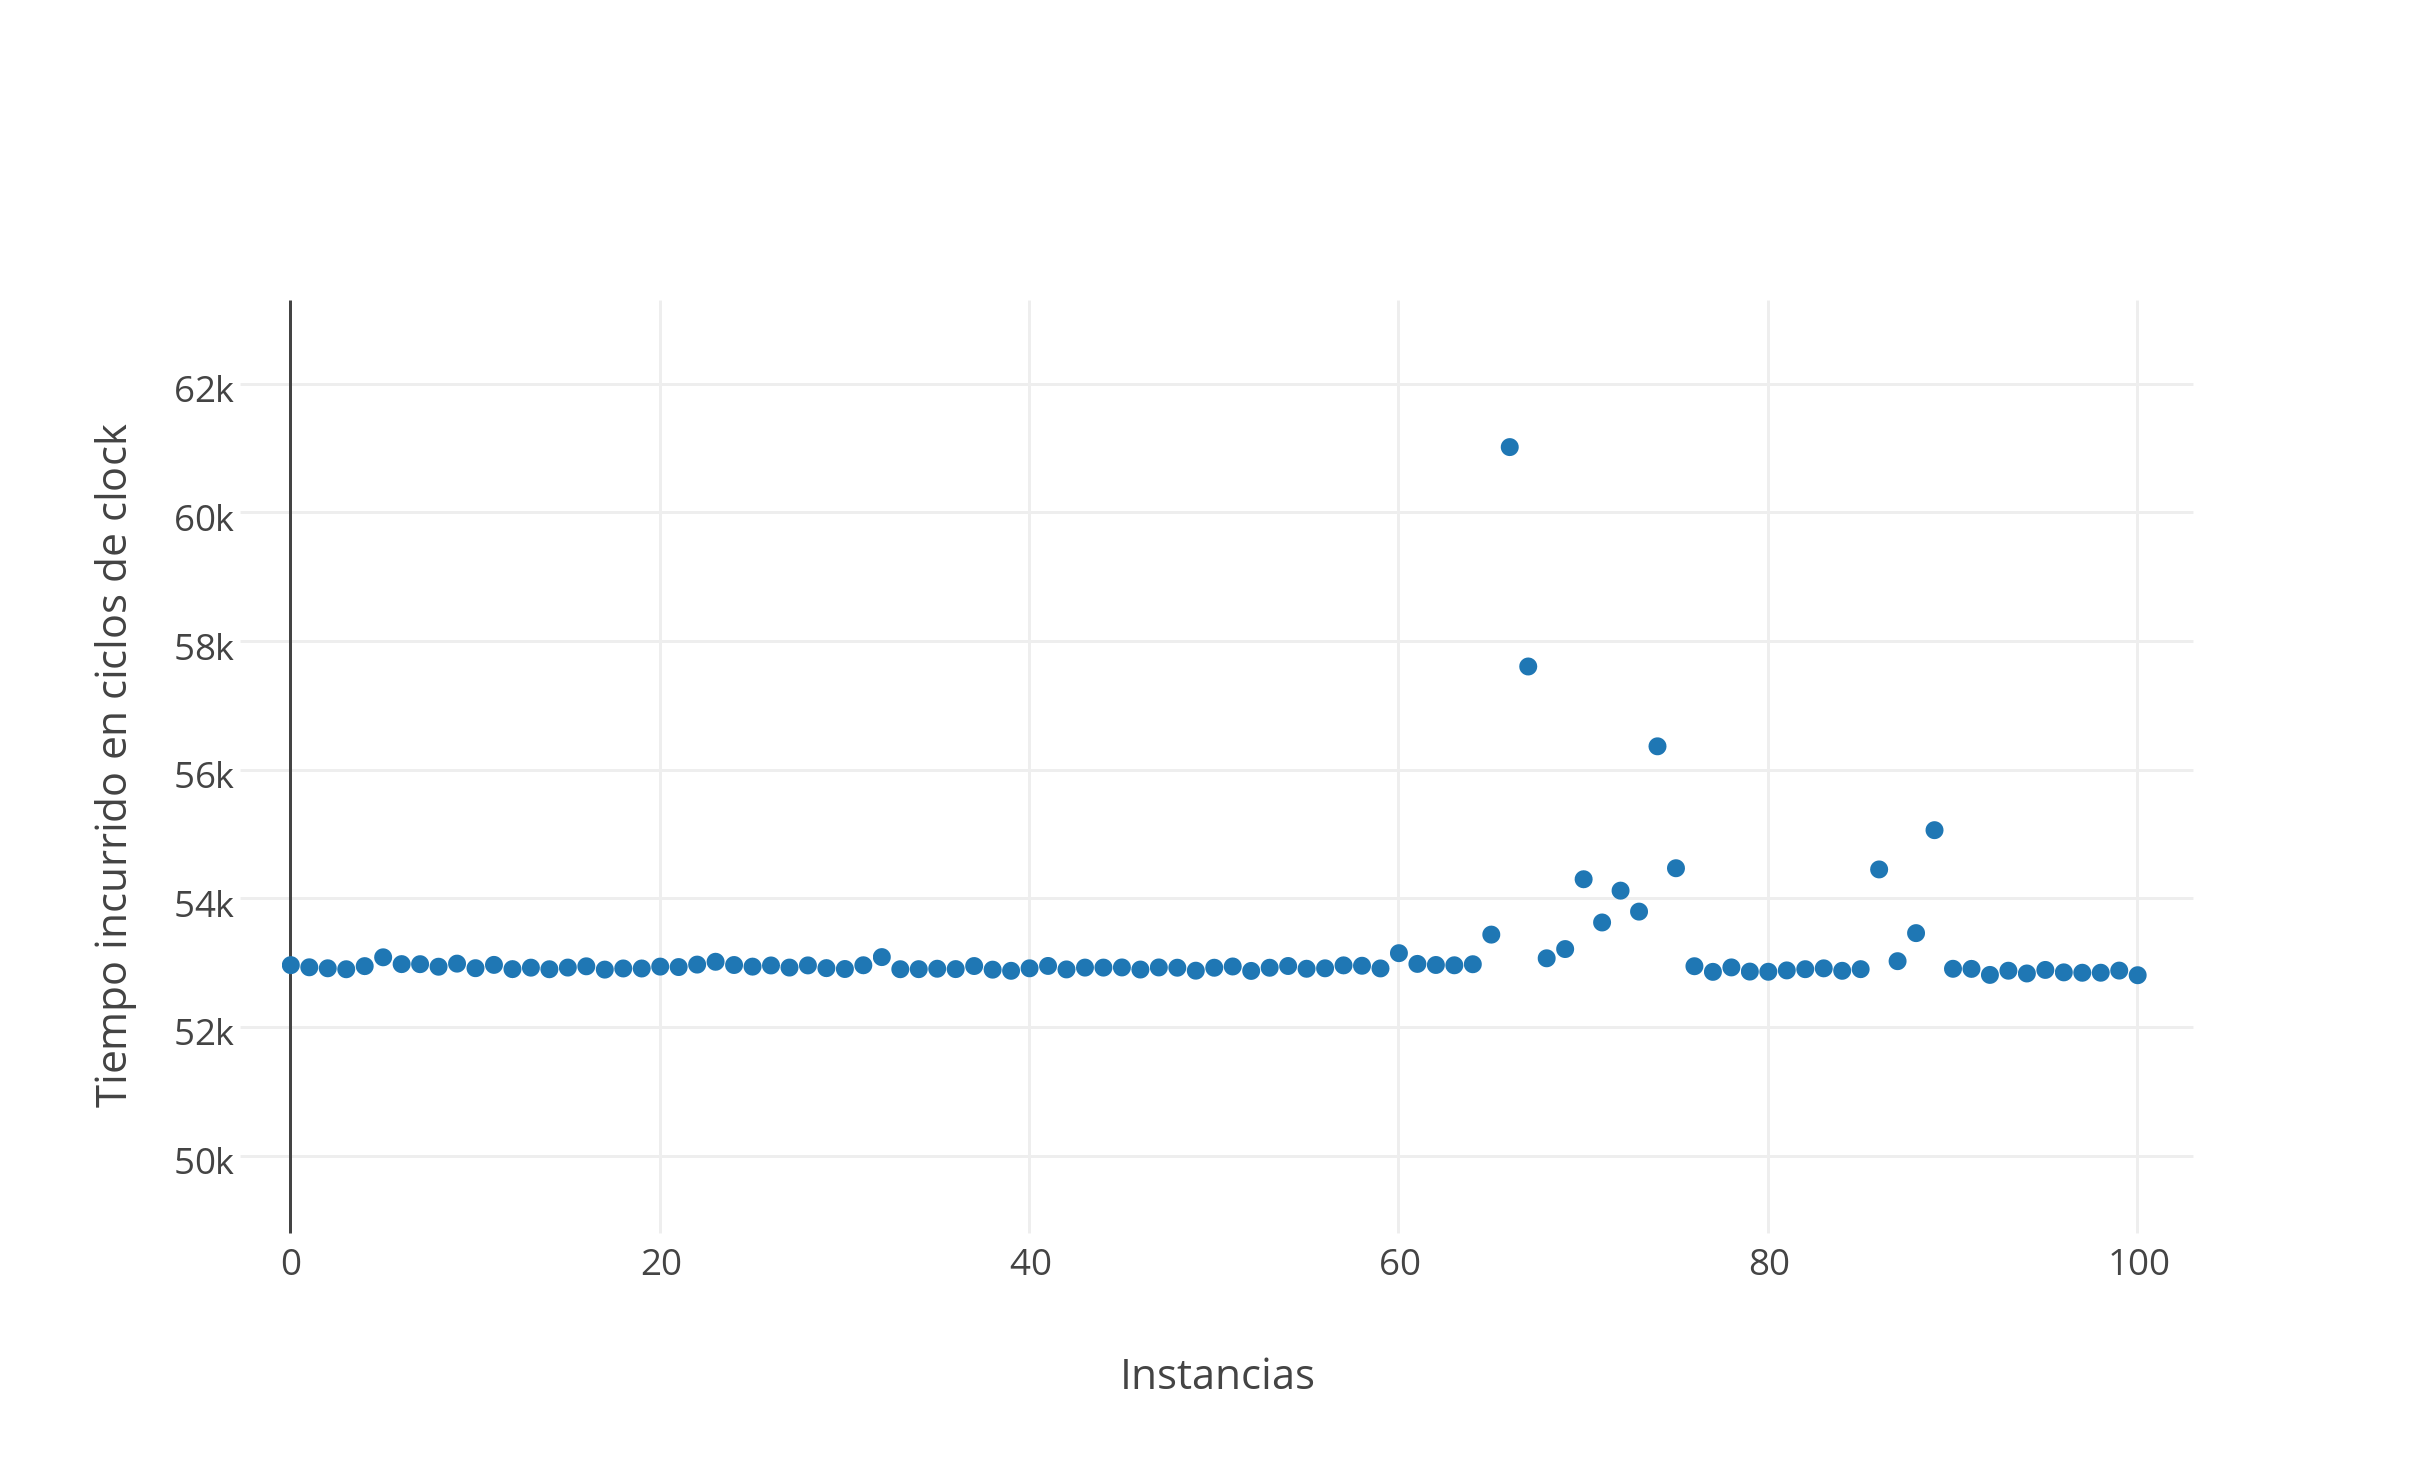
\includegraphics[scale=0.5]{imagenes/1C.png}
	\end{center}
	\caption{Dakkar - Variables constantes, instancias variables}\label{fig:1D}
\end{figure}

Podemos observar que manteniendo constantes todas las variables, pero alterando los tiempos de todas las etapas, no se pueden apreciar diferencias notables respecto al tiempo. Esto respalda nuestra teoría acerca de que nuestro algoritmo no depende de los valores, sino de las variables, (o sea que no parecería haber un mejor o peor caso temporal).